% Declare type of document
\documentclass[10pt]{article}

% Import Packages
\usepackage[utf8]{inputenc}

% Commonly used math symbols and fonts
\usepackage[mathscr]{euscript}
\usepackage{amsfonts,amsmath,amssymb,amsthm}
\usepackage{mathtools,mathdots}

% Better looking default font
\usepackage{lmodern}

% itemize environment
\usepackage{enumitem}

% Array, longtable, and booktabs
\usepackage{array}
\usepackage{longtable}
\usepackage{booktabs}

% Caption package for hiding Figure #
\usepackage{caption}

% Page formatting
\usepackage[letterpaper, margin=1in]{geometry}

% Package for nice syntax highlighting for code
\usepackage{minted}

% Allows line breaks in the math environment
\allowdisplaybreaks

\usepackage[activate={true,nocompatibility},final,tracking=true,kerning=true,spacing=true,factor=1100,stretch=10,shrink=10]{microtype}
\microtypecontext{spacing=nonfrench}
% activate={true,nocompatibility} - activate protrusion and expansion
% final - enable microtype; use "draft" to disable
% tracking=true, kerning=true, spacing=true - activate these techniques
% factor=1100 - add 10% to the protrusion amount (default is 1000)
% stretch=10, shrink=10 - reduce stretchability/shrinkability (default is 20/20)


\title{CS 310: Stack and Queue (Part I)}
\author{Connor Baker}
\date{February 12, 2019}

\begin{document}

\maketitle

\subsection*{Review}
\begin{itemize}
    \item \mintinline{java}{Iterator}s
    \begin{itemize}
        \item Motivation: why do we need iterators?
        \begin{itemize}
            \item They can provide a specialized and performant method of traversing over some list.
        \end{itemize}
        \item Implementation: how do we support efficient iterations?
        \begin{itemize}
            \item Use a nested class or an inner (anonymous) class. Doing so allows access to otherwise private members, and a deeper understanding of the internal workings of the class provides for a more efficient iterator (at the cost of higher coupling).
        \end{itemize}
    \end{itemize}
    \item Take-home
    \begin{itemize}
        \item When you use a data structure, use an \mintinline{java}{Iterator} to improve efficiency and uniformity
        \item When you design or implement a data structure, consider providing an \mintinline{java}{Iterator} for the above reason
    \end{itemize}
\end{itemize}


\subsection*{New Topic}
\begin{itemize}
    \item Stack
    \begin{itemize}
        \item A data structure that works like a stack (what a twist!)
    \end{itemize}
    \begin{center}
    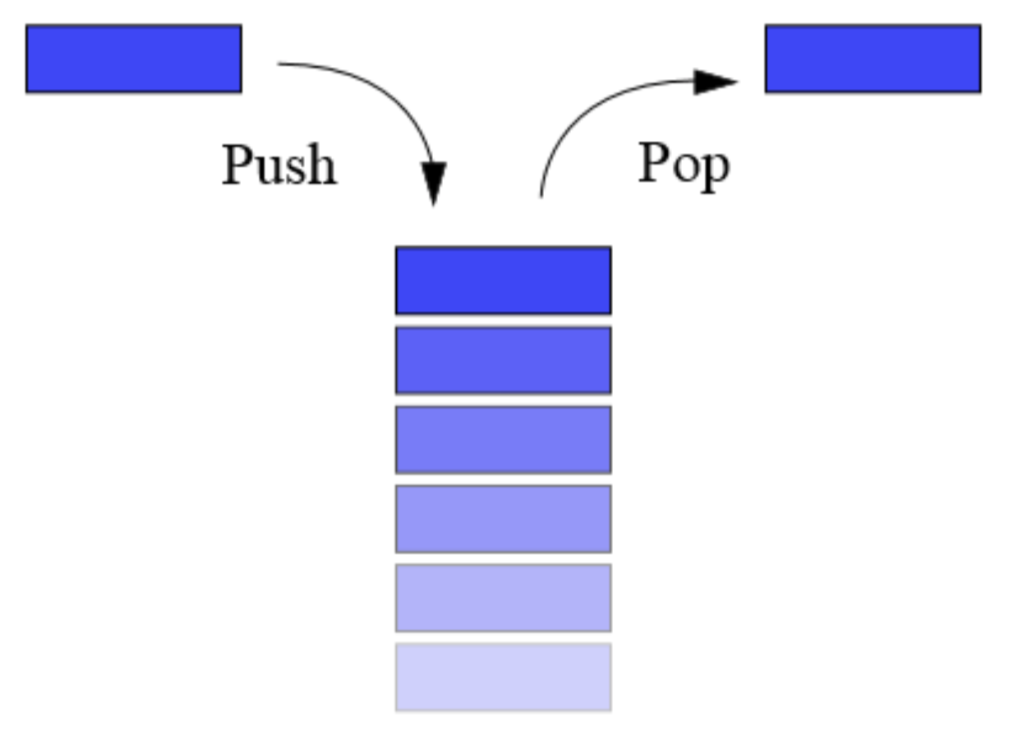
\includegraphics[width=\textwidth/3]{images/1.png}
    \end{center}
    \item Queue
    \begin{itemize}
        \item A data structure that works like people waiting in a line (or queue if you're British)
    \end{itemize}
    \begin{center}
    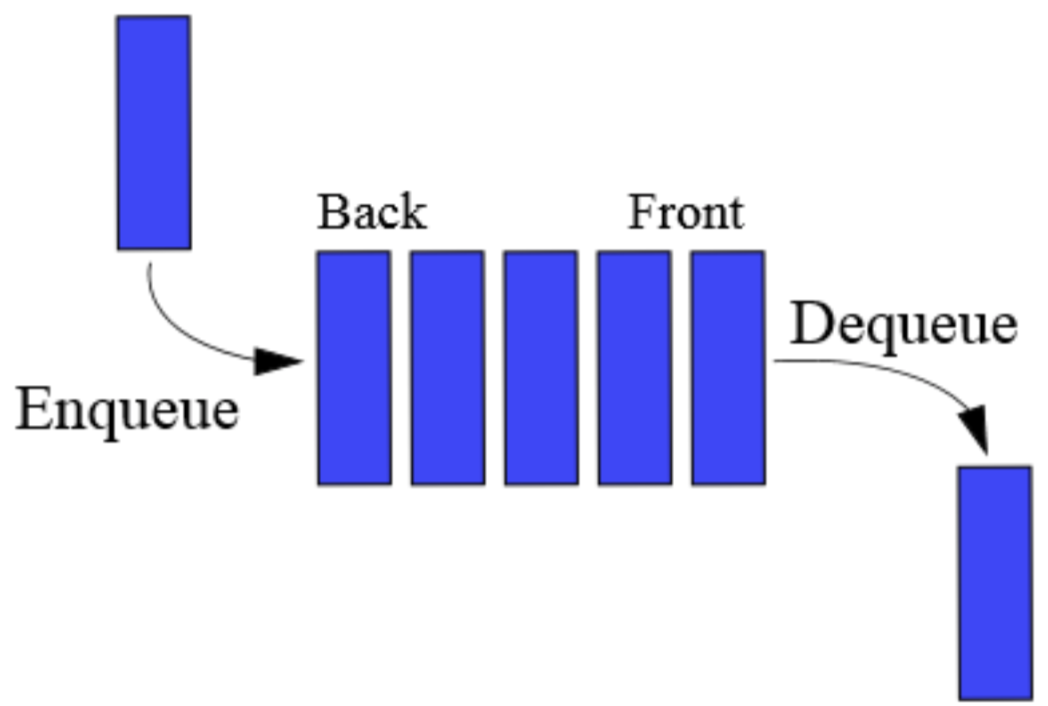
\includegraphics[width=\textwidth/3]{images/2.png}
    \end{center}
\end{itemize}


\subsection*{Stack}
\begin{itemize}
    \item Features
    \begin{itemize}
        \item LIFO
        \item Always operates at the top of the stack
    \end{itemize}
    \item Basic operations
    \begin{itemize}
        \item \mintinline{java}{.push(T t)}: add \mintinline{java}{t} to the top of the stack (grows the stack)
        \item \mintinline{java}{.pop()}: remove the top of the stack (shrinks the stack)
        \item \mintinline{java}{.top()}: return the top of the stack (size is not changed)
        \item \mintinline{java}{.isEmpty()}: true when nothing is in it, false otherwise
    \end{itemize}
    \item Implementation
    \begin{itemize}
        \item Based on array / linked list
    \end{itemize}
\end{itemize}
\begin{center}
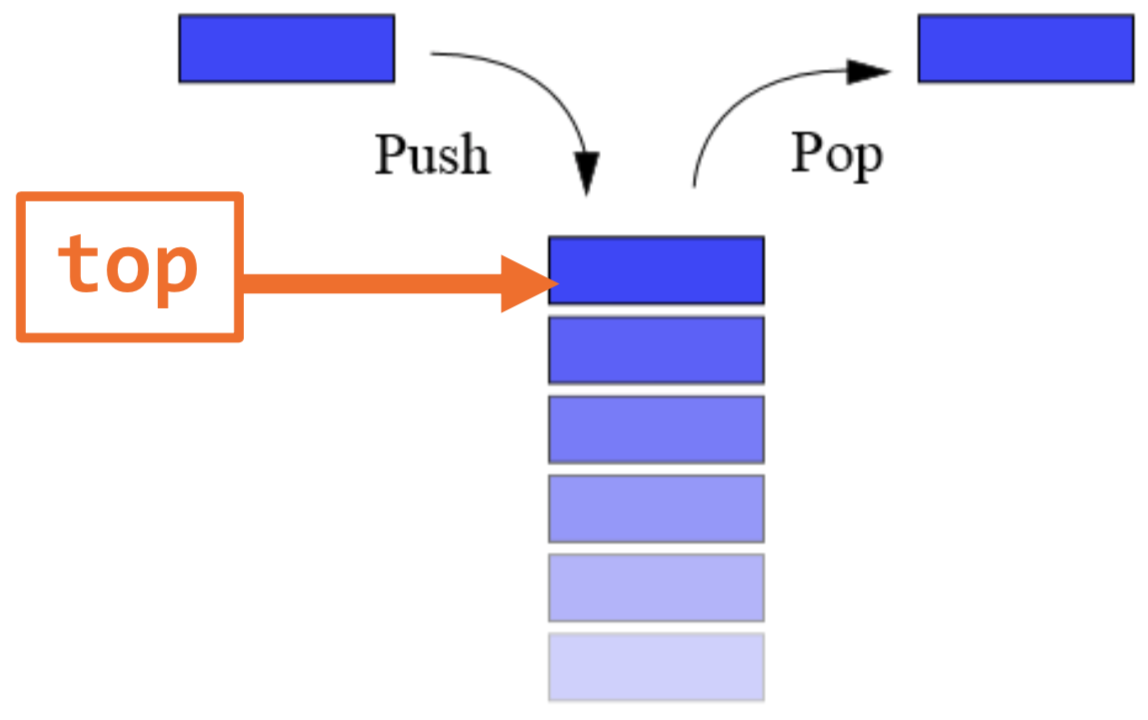
\includegraphics[width=\textwidth/3]{images/3.png}
\end{center}


\subsection*{Stack Example}
\begin{itemize}
    \item You need to be able to draw the stack contents
\end{itemize}
\begin{minted}{java}
s = new Stack();
s.push(4);
s.push(10);
s.push(5);
s.pop();
s.push(11);
\end{minted}

\subsection*{Stacks based on Arrays}
\begin{minted}{java}
class AStack<T>{
    private ArrayList<T> stuff; 
    public AStack(); // Constructor
    public void push(T x); // like add(x) or append(x)
    public void pop(); // like remove(size()-1)
    public T top(); // like get(size()-1)
    public boolean isEmpty(); // like size()==0
}
\end{minted}
\begin{itemize}
    \item Use an \mintinline{java}{ArrayList} as the underlying storage
    \item The top of the stack is the end of the array
    \begin{itemize}
        \item Operations are performed only at the end which makes it faster with an array based implementation
    \end{itemize}
    \item What's the Big-O?
    \begin{itemize}
        \item $O(1)$
    \end{itemize}
\end{itemize}

\subsection*{Stack Based on Linked List}
\begin{minted}{java}
Class LStack<T>{
    private LinkedList<T> stuff;
    public LStack(); // Assume head as stack top
    public void push(T x); // like insert(0,x)
    public void pop(); // like remove(0)
    public T top(); // like get(0)
    public boolean isEmpty(); // like size()==0
}
\end{minted}
\begin{itemize}
    \item Use a Linked List as the underlying storage
    \begin{itemize}
        \item Operate only at one end
    \end{itemize}
    \item Big-O?
    \begin{itemize}
        \item $O(1)$
    \end{itemize}
\end{itemize}
\begin{center}
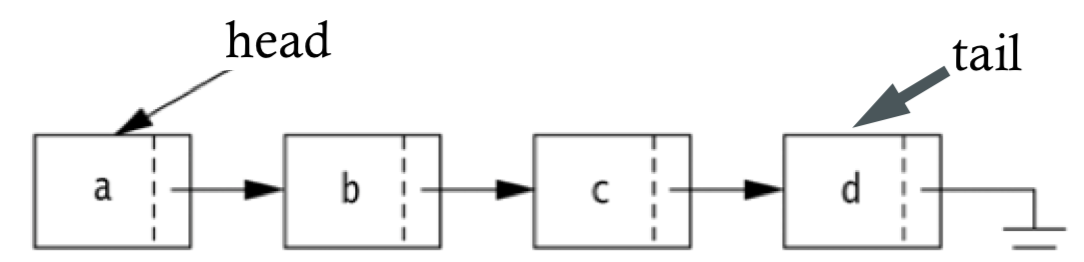
\includegraphics[width=\textwidth/2]{images/4.png}
\end{center}


\subsection*{Stack Applications}
\begin{itemize}
    \item Check the symbolic balancing of an equation
    \begin{itemize}
        \item $\{(<>[\{<>\}])\{\}\}$ vs. $\{(<[\{<>>\}])\{\}\}$
    \end{itemize}
    \item Postfix calculation
    \begin{itemize}
        \item $6\ 5\ 2\ 3\ +\ 8\ \times\ +\ 3\ +\ \times\ = $
    \end{itemize}
    \item Infix to Postfix conversion
    \begin{itemize}
        \item $a\ +\ b\ \times\ c\ +\ (d\ \times\ e\ +\ f)\ \times\ 
        g \to abc\ \times\ +\ de\ \times\ f\ +\ g\ \times\ +$
    \end{itemize}
    \item Call stack
    \begin{itemize}
        \item \mintinline{java}{fib(4)}
    \end{itemize}
    \item Tree traversal -- preorder traversal
    \item Graph search -- depth first search
    \item And a bunch of over applications
\end{itemize}

\subsection*{Queue}
\begin{itemize}
    \item Features
    \begin{itemize}
        \item FIFO
        \item Only remove from front
        \item Only add to back
    \end{itemize}
    \item Basic operations
    \begin{itemize}
        \item \mintinline{java}{.enqueue(T t)} or \mintinline{java}{.add(T t)}: \mintinline{java}{t} enters at the back
        \item \mintinline{java}{.dequeue()} or \mintinline{java}{.poll()}: front leaves
        \item \mintinline{java}{.getFront()} or \mintinline{java}{.peek()}: returns the item at the front
        \item \mintinline{java}{.isEmpty()}: true when nothing is in it, false otherwise
    \end{itemize}
\end{itemize}

\begin{center}
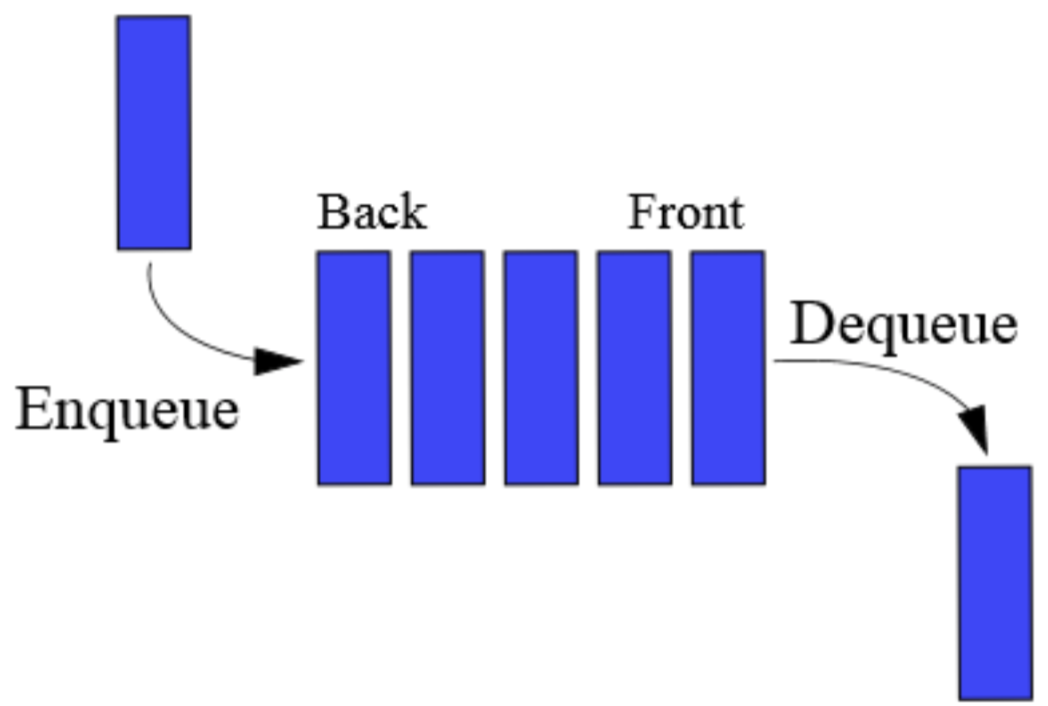
\includegraphics[width=\textwidth/3]{images/2.png}
\end{center}



\subsection*{Queue Example}
\begin{itemize}
    \item You need to be able to draw the queue contents
    \item What is the value of \mintinline{java}{v}?
\end{itemize}
\begin{minted}{java}
q = new Queue(); // Empty queue
q.enqueue(4); // 4
q.enqueue(10); // 4 10
q.enqueue(5); // 4 10 5
q.dequeue(); // 10 5
v = getFront(); // v == 10
q.dequeue(); // 5
q.enqueue(11); // 5 11
q.enqueue(25); // 5 11 25
\end{minted}

\subsection*{Queue Based on Linked Lists}
\begin{center}
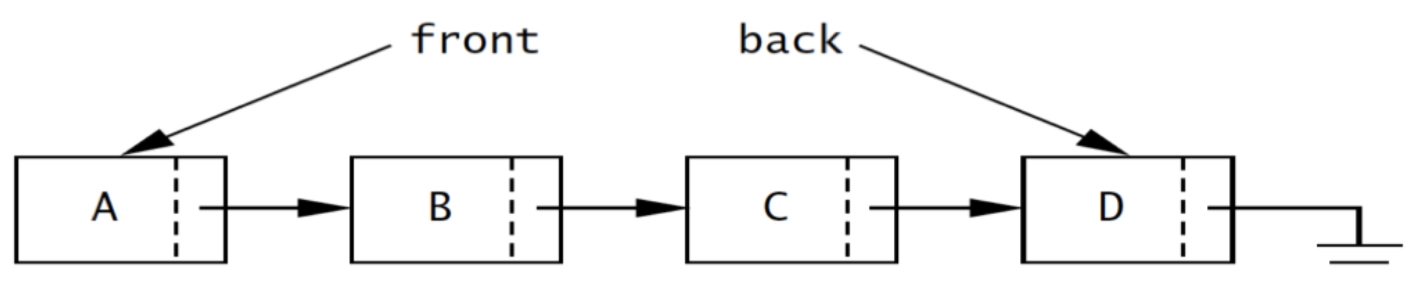
\includegraphics[width=\textwidth/2]{images/5.png}
\end{center}
\begin{itemize}
    \item Append to one end, and remove from the other end
    \begin{itemize}
        \item For example, \mintinline{java}{head}$\to$\mintinline{java}{front}, \mintinline{java}{tail}$\to$\mintinline{java}{back}
        \item \mintinline{java}{.enqueue(T t)}: insert at the tail
        \item \mintinline{java}{.dequeue()}: remove from head
        \item \mintinline{java}{.getFront()}: return head contents
        \item \mintinline{java}{.isEmpty()}: \mintinline{java}{.size() == 0}
    \end{itemize}
\end{itemize}

\subsection*{Queue Based on Arrays}
\begin{itemize}
    \item Naive implementation:
    \begin{itemize}
        \item \mintinline{java}{.enqueue(T t)}: insert at the end
        \item \mintinline{java}{.dequeue()}: remove from start and shifting internally
        \begin{itemize}
            \item In fact, a \textit{lot} of shifting! Shifting is done for every single \mintinline{java}{.dequeue()}!
        \end{itemize}
        \item Alternatively, we could just mark the front and the back in the array and update them with \mintinline{java}{.enqueue()} and \mintinline{java}{.dequeue()}
    \end{itemize}
\end{itemize}


\subsection*{Queue Based on Arrays}
\begin{center}
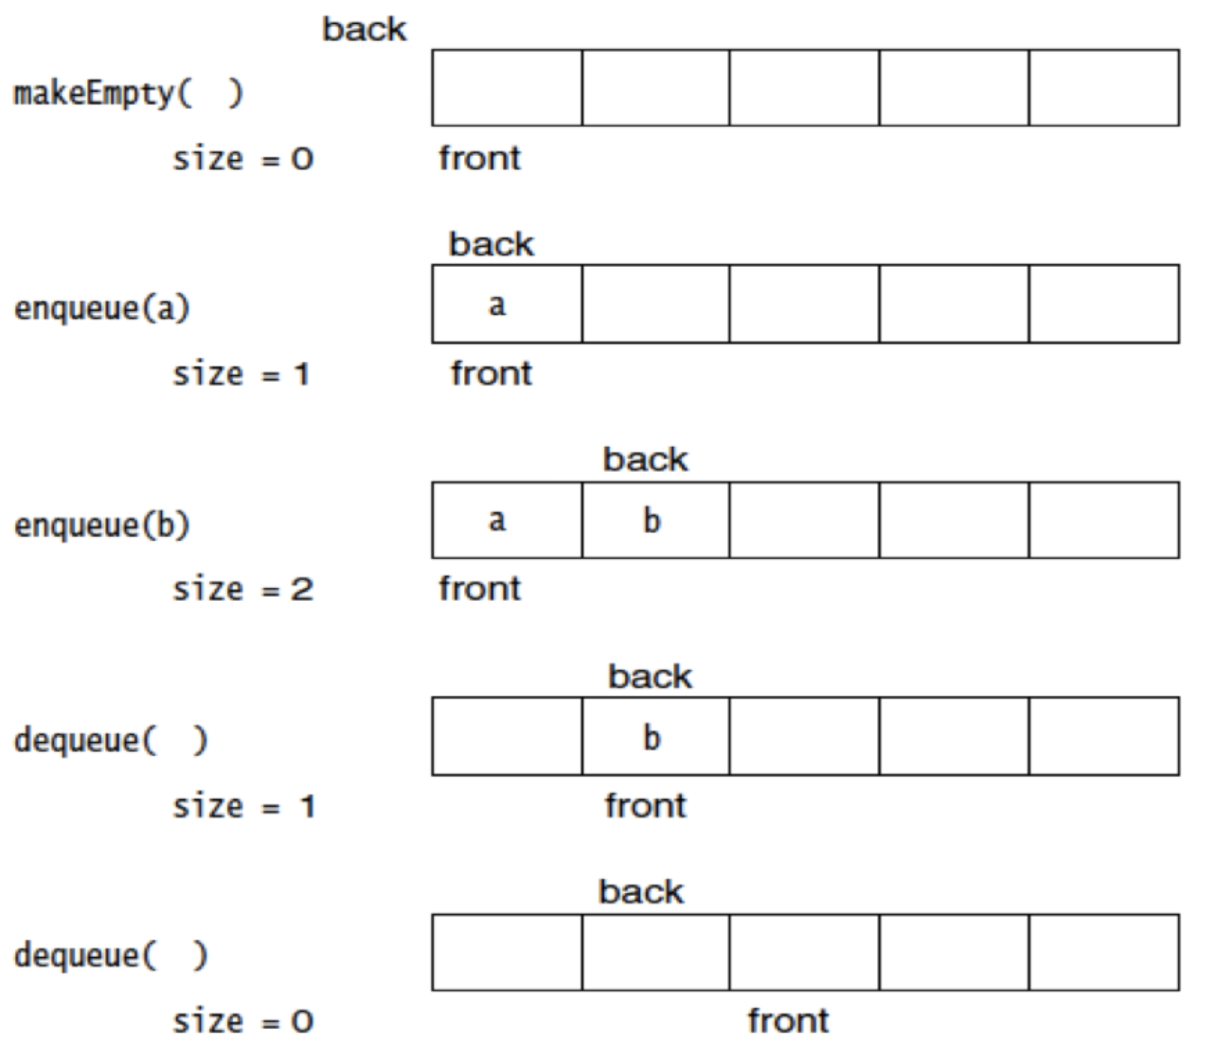
\includegraphics[width=\textwidth/2]{images/6.png}
\end{center}
\begin{itemize}
    \item Between the front and the back, we have a valid queue
    \begin{itemize}
        \item There's no shifting: $O(1)$ for \mintinline{java}{.dequeue()}!
        \item But it does use a sizeable amount of space -- this makes it a good structure for fixed size queues
    \end{itemize}
\end{itemize}

\subsection*{Queue: Array with Wraparound}
\begin{center}
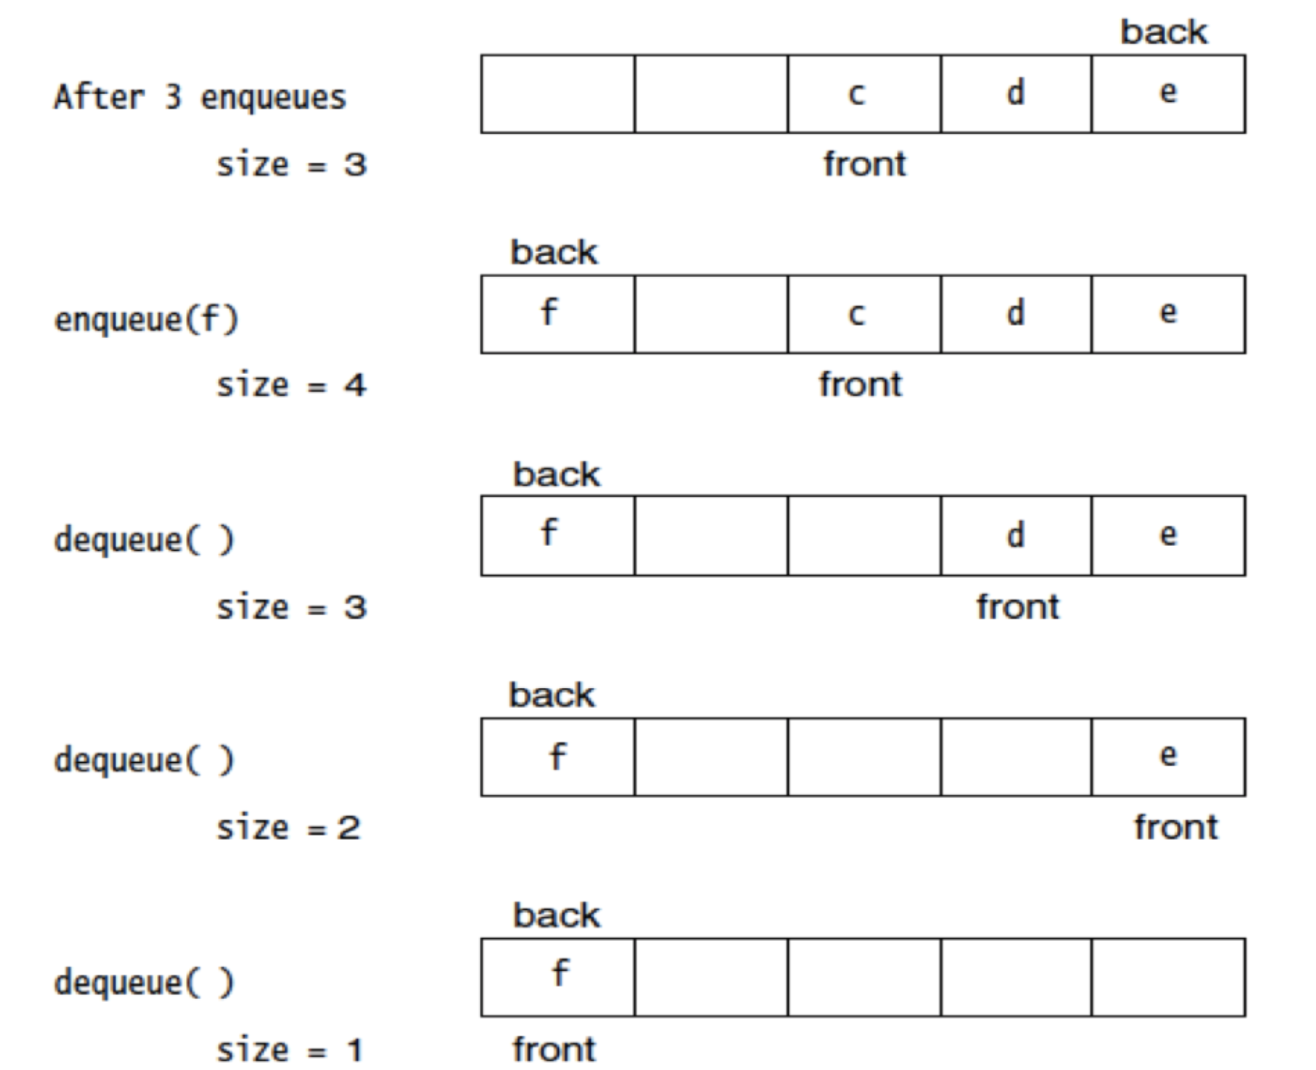
\includegraphics[width=\textwidth/2]{images/7.png}
\end{center}
\begin{itemize}
    \item Exercise: what needs to be changed to implement the wraparound functionality?
    \begin{itemize}
        \item Our mutator and accessor methods -- unless we do all of these through an iterator, in which case only the iterators understanding of its position relative to the front and end of the queue need to change.
    \end{itemize}
\end{itemize}

\subsection*{Big-O Comparison}
\begin{itemize}
    \item Stack
\end{itemize}
\begin{center}
    \begin{tabular}{lccccr} \toprule
        Implementation & \mintinline{java}{.push()} & \mintinline{java}{.pop()} & \mintinline{java}{.top()} & \mintinline{java}{.isEmpty()} & \mintinline{java}{.size} \\ \midrule
        Array & 1$^*$ & 1 & 1 & 1 & 1 \\
        Linked List & 1 & 1 & 1 & 1 & 1 \\ \bottomrule
    \end{tabular}
    \begin{center}*Amortized analysis\end{center}
\end{center}
\begin{itemize}
    \item Queue
\end{itemize}
\begin{center}
    \begin{tabular}{lccccr} \toprule
        Implementation & \mintinline{java}{.enqueue()} & \mintinline{java}{.dequeue()} & \mintinline{java}{.getFront()} & \mintinline{java}{.isEmpty()} & \mintinline{java}{.size} \\ \midrule
        Array & 1$^*$ & 1 & 1 & 1 & 1 \\
        Linked List & 1 & 1 & 1 & 1 & 1 \\ \bottomrule
    \end{tabular}
    \begin{center}*Amortized analysis\end{center}
\end{center}

\subsection*{Why use a Stack or Queue}
\begin{itemize}
    \item Restricted operations give us good worst cases
    \begin{itemize}
        \item $O(1)$ for all supported operations
        \item $O(n)$ for space
    \end{itemize}
    \item Simple data structures
    \begin{itemize}
        \item Focus on limited operations
        \item Can be made out of primitive data structures (arrays and linked lists)
    \end{itemize}
    \item Good for representing time-related data
    \begin{itemize}
        \item Call stack
        \item Packet queues
    \end{itemize}
\end{itemize}

\subsection*{Review: Queues}
\begin{itemize}
    \item FIFO
    \item Supported operations:
    \begin{itemize}
        \item \mintinline{java}{.enqueue(x)}: insert at the tail
        \item \mintinline{java}{.dequeue()}: remove from head
        \item \mintinline{java}{.getFront()}: return head contents
        \item \mintinline{java}{.size()}: returns the size of the queue
        \item \mintinline{java}{.isEmpty()}
    \end{itemize}
    \item Applications:
    \begin{itemize}
        \item Simulate a process with a FIFO order
        \item Scheduling queue of a CPU or disk or printer
        \item Serve as a buffer for file I/O, network communications, etc.
    \end{itemize}
\end{itemize}

\subsection*{Priority Queues}
\begin{itemize}
    \item Much of the time tasks that we use a queue for have different priorities
    \begin{itemize}
        \item It is convention that the lower the priority, the better
        \item Symmetric code if higher is better
        \item Dequeue the ones with the ``best" priority first
    \end{itemize}
    \item Common priority queue operations
    \begin{itemize}
        \item \mintinline{java}{void insert(T t, int p)}: insert \texttt{t} with priority \texttt{p}
        \item \mintinline{java}{T findMin()}: return the object with the ``best" priority
        \item \mintinline{java}{void deleteMin()}: remove the object with the ``best" priority
    \end{itemize}
\end{itemize}

\subsection*{Priority Queue Design}
\begin{center}
    \begin{tabular}{lcccr} \toprule
        Data Structure & \mintinline{java}{.insert()} & \mintinline{java}{.findMin()} & \mintinline{java}{.deleteMin()} & Notes \\ \midrule
        Sorted Array & $O(n)$ & $O(1)$ & $O(1)$ & min at high index \\
        Sorted Linked List & $O(n)$ & $O(1)$ & $O(1)$ & min at head or tail \\ \bottomrule
    \end{tabular}
\end{center}
\begin{itemize}
    \item Other data structures exist as good candidates of priority queues
    \begin{itemize}
        \item Binary search trees
        \item Heaps
        \item We'll cover these later
    \end{itemize}
\end{itemize}


\subsection*{Summary}
\begin{itemize}
    \item Stacks and queues
    \begin{itemize}
        \item Try implementing them
        \item Project 2
    \end{itemize}
    \item Next lecture: Trees, recursion
    \begin{itemize}
        \item Reading: Chapter 18, Chapter 7
    \end{itemize}
\end{itemize}


\end{document}